%!TEX TS-program = xelatex 
%!TEX TS-options = -synctex=1 -output-driver="xdvipdfmx -q -E"
%!TEX encoding = UTF-8 Unicode
%
%  transparency
%
%  Created by Mark Eli Kalderon on 2014-07-08.
%  Copyright (c) 2014. All rights reserved.
%

\documentclass[12pt]{article} 

% Definitions
\newcommand\mykeywords{Aristotle, transparency}
\newcommand\myauthor{Mark Eli Kalderon}

% Packages
\usepackage{geometry} \geometry{a4paper} 
\usepackage{url}
\usepackage{txfonts}
\usepackage{color}
\usepackage{enumerate}
\definecolor{gray}{rgb}{0.459,0.438,0.471}
\usepackage{setspace}
% \doublespace % Uncomment for doublespacing if necessary
% \usepackage{epigraph} % optional

% XeTeX
\usepackage[cm-default]{fontspec}
\usepackage{xltxtra,xunicode}
\defaultfontfeatures{Scale=MatchLowercase,Mapping=tex-text}
\setmainfont{Hoefler Text}

% Bibliography
\usepackage[round]{natbib}

% Title Information
\title{Aristotle on Transparency}
\author{\myauthor} 
\date{} % Leave blank for no date, comment out for most recent date

% PDF Stuff
\usepackage[plainpages=false, pdfpagelabels, bookmarksnumbered, backref, pdftitle={Form Without Matter}, pagebackref, pdfauthor={\myauthor}, pdfkeywords={\mykeywords}, xetex, colorlinks=true, citecolor=gray, linkcolor=gray, urlcolor=gray]{hyperref} 

%%% BEGIN DOCUMENT
\begin{document}

% Title Page
\maketitle
% \begin{abstract} % optional
% \noindent
% \end{abstract} 
% \vskip 2em \hrule height 0.4pt \vskip 2em
% \epigraph{text of epigraph}{\textsc{author of epigraph}} % optional; make sure to uncomment \usepackage{epigraph}

% Layout Settings
\setlength{\parindent}{1em}

% Main Content

\section{An unpromising topic?} % (fold)
\label{sec:an_unpromising_topic_}

Aristotle on transparency can seem like an unpromising topic. Many commentators have been unkind. Some commentators have suggested that Aristotle's account is of antiquarian interest only. Others have expressed incredulity at the way Aristotle's account conflicts with the manifest facts of experience. So why write about Aristotle on transparency?

In a transparent medium, such as air or water, objects can appear in or through that medium. This is a remarkable fact. (Though, perhaps, one we may have grown jaded about in our hypervisual culture). As we shall see, this remarkable fact about transparency is bound up with an ancient puzzle or \emph{aporia} about the nature of sensory presentation at work in color vision. This puzzle animates Empedocles' account of color vision. Moreover, as I argue at length in (ref), Aristotle's notorious definition of perception as the assimilation of the sensible form of an object without its matter is a dialectical response to this puzzlement. 

% section an_unpromising_topic_ (end)

\section{A puzzle about perception at a distance} % (fold)
\label{sec:a_puzzle_about_perception_at_a_distance}

In \emph{La Dioptrique}, Descartes makes the striking and paradoxical comparison between vision and a blind man's use of sticks in navigation, a kind of haptic touch (see Figure~\ref{fig:blind}). The analogy is, in fact, an ancient one. Alexander of Aphrodisias attributes it to the Stoics (\emph{De Anima} 130 14). The Stoic analogy was criticized by Galen in \emph{De Placitis Hippocratis et Plotonis} 2.5, 2.7, and by Tideus in \emph{De Speculis}. Though an ancient analogy, Descartes makes distinctively modern use of it. Thus, for example, Descartes not only uses the analogy to motivate his mechanical account of vision but also in support of the claim that there need be nothing in objects that resemble the ideas or sensations that we have of them. Just as the Stoic use of the analogy had its critics, so too the Cartesian use. Thus Merleau-Ponty complains:
\begin{quote}
	The blind, says Descartes, ‘see with their hands’. Cartesian concept of vision is modeled after the sense of touch. At one swoop, then, he removes action at a distance and relieves us of that ubiquity which is the whole problem of vision (as well as its peculiar virtue). \citep[170]{Merleau-Ponty:1964aa}
\end{quote}

\begin{figure}[htbp]
	\centering
		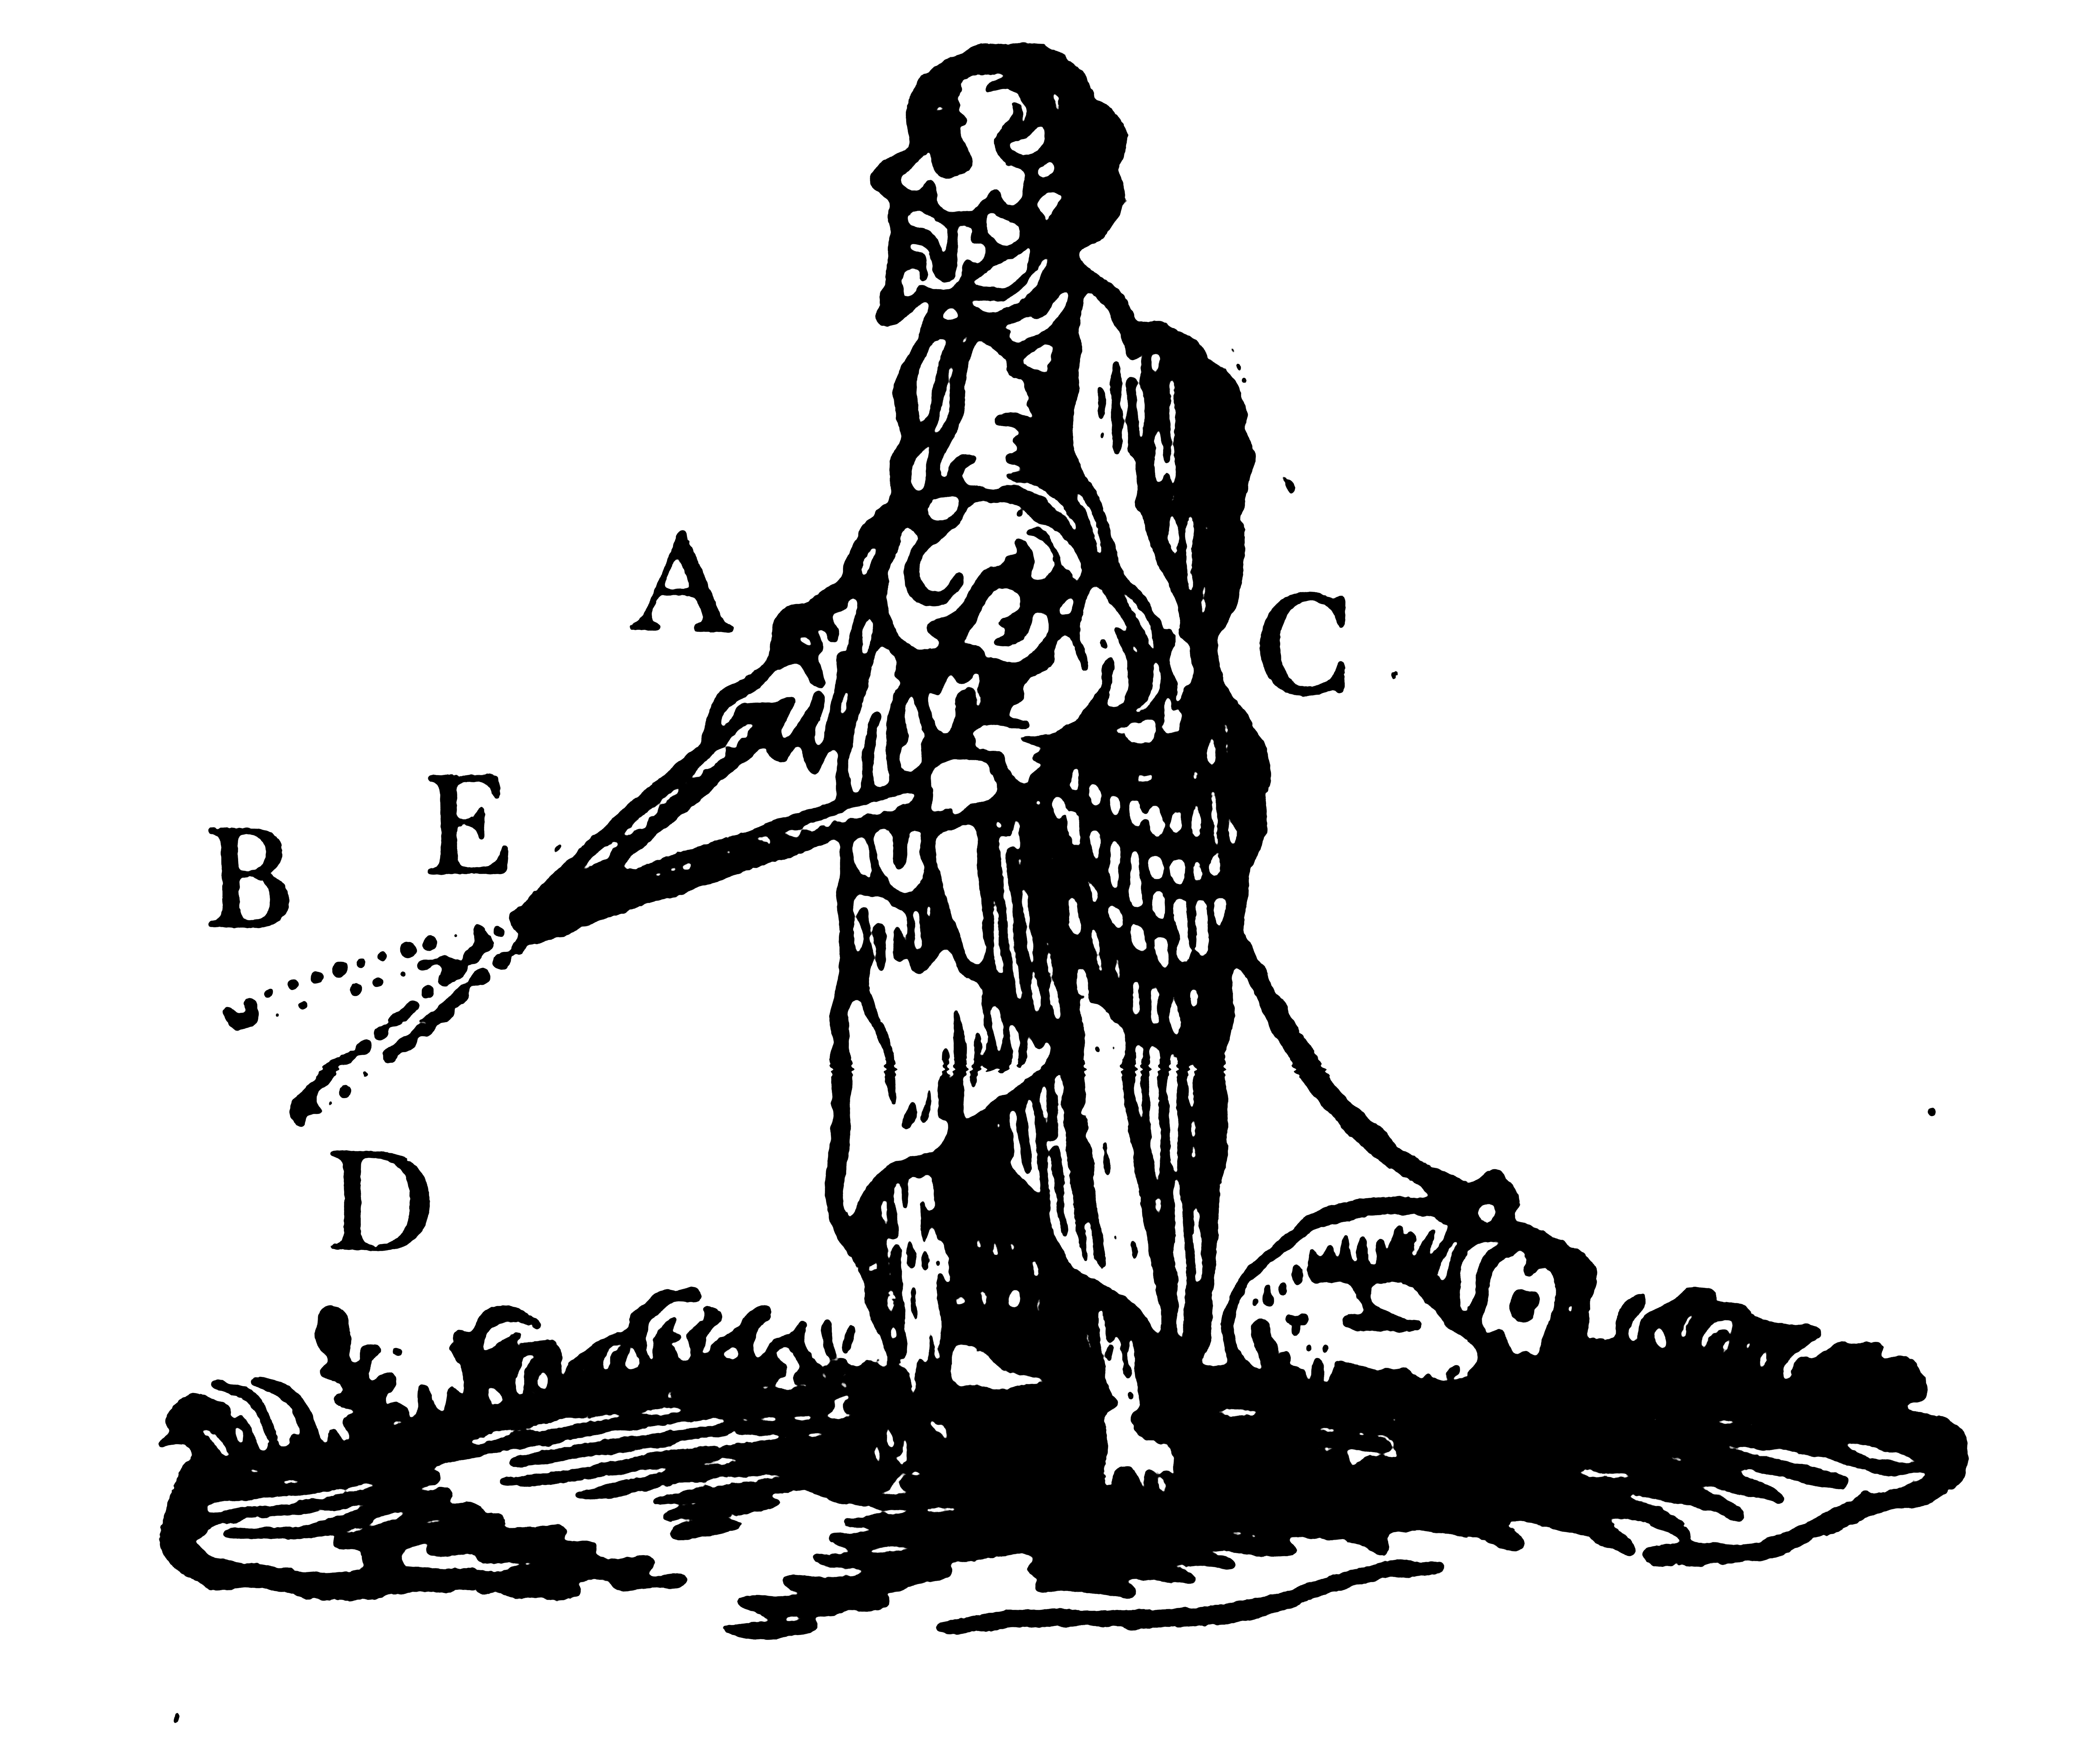
\includegraphics[scale=2]{graphics/blind.jpeg}
	\caption{\citealt{Descartes:1637uq}}
	\label{fig:blind}
\end{figure}

What is it about vision that constitutes the whole problem of vision as well as its peculiar virtue? Merleau-Ponty describes vision as a kind of action at a distance. This can suggest that the problem concerns the causal mechanisms that underly visual perception. Suppose vision is a kind of action at a distance. A problem would arise if one further held that causation, or at least immediate causation, requires contact. If causation requires contact, there is no action at a distance. This is misleading, however. Given the state of optical knowledge even at the time of Merleau-Ponty's writing, there was no serious question whether visual perception involved action at a distance in this sense. Light reflected, transmitted, and emitted from the scene travels to the perceiver and so irradiates their sensory surfaces, in Quine's \citeyearpar{Quine:1960rm} deflationary locution. 

In speaking of vision as a kind of action at a distance, Merleau-Ponty was not denying the existence of a proximal cause for vision, rather he was making a phenomenological observation, that vision presents us with objects located at a distance. That vision presents us with objects located at a distance, that vision is a mode of awareness of the distal environment, is plausibly that in which its peculiar virtue consists. Thus Aristotle claims that by means of vision animals capable of locomotion may move towards sources of vital nourishment just as they may flee mortal danger (\emph{De Anima} \textsc{iii} 12 434\( ^{a} \)81--82). Describing the ability to see objects located at a distance as the peculiar virtue of vision perhaps overstates the case. Audition is a distal sense as well. One may hear a distant predator just as one may see it. However, it remains easy to appreciate the utility of vision presenting objects located at a distance. 

The ubiquity which is the whole problem of vision concerns less the causal mechanisms that underly the presentation in vision of objects located at a distance than with the nature of their visual presentation. An Aristotelian might suggest, on Merleau-Ponty's behalf, that action in the slogan ``action at a distance'' refers less to the object of perception acting upon the perceiver, whether mediately or immediately, than to perceptual activity, understood as \emph{energeia}, the seeing of the object. Since the exercise of our visual capacity is the presentation in visual perception of the distal object, then action at a distance would instead refer to the visual presentation of an object located at a distance. Whether or not and to what extent Merleau-Ponty would have accepted the Aristotelian suggestion, the conclusion which we have reached by means of it, that the ubiquity which is the whole problem of vision concerns the visual presentation of objects located at a distance, is an understanding of that problem genuinely shared with Merleau-Ponty.

What is potentially problematic about the visual presentation of objects located at a distance? Given that the whole problem of vision concerns the presentation of objects located at a distance, somehow the distal character of the visible object must be inconsistent or at least in tension with the claim that it is presented in visual experience, on a compelling or at least plausible conception of visual presentation. The problem is usefully developed in terms of Broad's discussion of vision in ``Some elementary reflections on sense-perception''. There he writes:
\begin{quote}
	In its purely phenomenological aspect \emph{seeing} is ostensibly \emph{saltatory}. It seems to leap the spatial gap between the percipient's body and a remote region of space. Then, again, it is ostensibly \emph{prehensive} of the surfaces of distant bodies as coloured and extended, and of external events as colour-occurrences \emph{localized} in remote regions of space. \citep[5]{Broad:1952kx}
\end{quote}

Vision is saltatory at least in the sense that objects located at a distance and their visible qualities and relations are present in our visual experience of them. So understood, this is just the phenomenological observation that Merleau-Ponty urged against the Cartesian use of the Stoic analogy. As we shall see, it is accepted too by Aristotle, though the Stagirite would reject the suggestion that visual awareness ``leaps'' the spatial gap between the perceiver and the object seen; rather, we peer through the gap (see \ref{}). 

Not only does Broad emphasize that visual perception presents us with aspects of the distal environment, in addition, he offers us a characterization of visual presentation as prehensive. ``Prehension'' belongs to a primordial family of tactile metaphors for perceptual awareness that include ``grasping'', ``apprehending''. All are modes of assimilation, and ``ingestion'' is a natural variant \citep[see][7]{Johnston:2006uq,Price:1932fk}. \citet{Burnyeat:1979mv} observes that assimilation as a metaphor for perception is inscribed in the history of the English language. The word ``perception'' derives from the Latin \emph{perceptio} meaning to take in, or assimilate. To think of visual presentation as prehensive, is to thing of seeing as taking in the seen before one.

It is easy to see how visual presentation conceived as a mode of prehension can seem to conflict with its saltatory character. It is natural to think of seeing as taking in the scene before one. But how can one take in what remains external? And if one can, what does taking in here mean such than one could? This puzzlement does not go un-noted by Broad:
\begin{quote}
	It is a natural, if paradoxical, way of speaking to say that seeing seems to `bring us into \emph{contact} with \emph{remote} objects' and to reveal their shapes and colors. \citep[33]{Broad:1952kx}
\end{quote}
It is this puzzlement which is the ubiquity which is the whole problem of vision as well as its peculiar virtue. Or so I suggest. Unsurprisingly, this puzzlement has ancient roots. It animates Empedocles' theory of vision, and motivates, in part, Aristotle's interest in the transparent.

% section a_puzzle_about_perception_at_a_distance (end)

\section{Empedocles and the answer in the style of Gorgias} % (fold)
\label{sec:empedocles_and_the_answer_in_the_style_of_gorgias}

In the \emph{Meno} Socrates attributes to Empedocles a conception of perception as a mode of assimilation of material effluences:
\begin{quotation}
    \textsc{meno}: And how do you define color?
    
    \ldots
    
    \textsc{socrates}: Would you like an answer in the style Gorgias, such as you most readily follow?
    
    \textsc{meno}: Of course I should.
    
    \textsc{socrates}: You and he believe in Empedocles' theory of effluences, do you not?
    
    \textsc{meno}: Wholeheartedly.
    
    \textsc{socrates}: And passages in which and through which the effluences make their way?
    
    \textsc{meno}: Yes.
    
    \textsc{socrates}: Some of the effluences fit into some of the passages whereas others are too great or too small.
    
    \textsc{meno}: That is right.
    
    \textsc{socrates}: Now you recognize the term `sight'?
    
    \textsc{meno}: Yes.
    
    \textsc{socrates}: From these notions, then, `grasp what I would tell,' as Pindar says. Color is an effluence from shapes commensurate with sight and perceptible to it. (\emph{Meno} 76\( ^{a-d} \))
\end{quotation}

The main elements of the account are relatively clear. Objects emit material effluences. Effluences are fine bodies that are kind differentiated in terms of magnitude. There are passages in which and through which material effluences may flow. Whether a material effluence may enter a passage depends on its magnitude. The magnitudes of some kinds of material effluences are too great or too small for them to flow through a given passage. Such passages exist in the membrane of the eye, thus allowing the eye to assimilate only a certain kind of material effluence, that is, the kind whose magnitude permits entry in ocular passages.

Thus we arrive at the answer in the style of Gorgias. That answer has three components. It specifies a kind of thing and two conditions that must be satisfied for a thing of that kind to be color. Color is (1) a kind of material effluence that is (2) commensurate with sight and (3) perceptible. First, color is a kind of material effluence, a chromatic effluence, say. Since material effluences are kind differentiated by magnitude, chromatic effluences have a distinctive magnitude. Second, chromatic effluences are commensurate with sight insofar as their distinctive magnitude permits entry in the passages of the membrane of the eye, the organ of sight. Notice, however, the assimilation of chromatic effluences by the organ of sight is not, by itself, the sensing of colors, otherwise the final condition would be redundant. The assimilation of chromatic effluence is at best a material precondition for their sensing. The thought seems to be this: In order for the chromatic effluences to be the object of sense, they first must be assimilated by the organ of sensation. It is only by assimilating chromatic effluences that they are presented to sight and are thereby seen. Socrates claims that the answer in the style of Gorgias may be generalized to the other sensory objects such as sound and smell. If that is right, then Empedocles, at least as presented by Socrates, is in the grip of a general conception of sensory awareness for which ingestion provides the model. Compare---in eating an olive, the matter of the olive is taken in and presented to the organ of taste and thereby tasted. On the ingestion model, to be perceptible is to be palpable to sense.

To be perceptible is to be palpable to sense. If one began with that thought, a puzzle would naturally arise about vision, for vision seems to present the colors of distant objects. Color perception seems to involve the presentation of color qualities inhering in bounded particulars located at a distance from the perceiver. But how can one assimilate what remains inherent in a bounded particular remote from one? The puzzlement arise from the apparent tension between two claims:
\begin{enumerate}[(1)]
    \item The objects of color perception are qualities of external particulars located at a distance from the perceiver.
    \item \emph{The Empedoclean principle}: To be perceptible is to be palpable to sense---in order for something to be the object of perception it must be in contact with the relevant sense organ.
\end{enumerate}

I conjecture that, whatever independent reasons Empedocles may have had for believing in material effluences, it is precisely this puzzlement that effluences are meant to address in his theory of vision. The basic idea is simple enough, at least in broad outline. Distant objects may be sensed by sensing the material effluences they emit. If the color of an object is the material effluence that it emits, then the color of a remote object can be assimilated and so be palpable to sight. In this way, we can see the color of a bounded particular remote from us  consistent with the constraints imposed by the ingestion model. One may wonder whether the theory of effluences is wholly adequate to this task, at least without supplementation. Thus a Berkelean worry naturally arises about the immediate objects of sensation, the assimilated effluences, screening off the external objects that emit them. Moreover, it is not just colored objects that appear at a distance, but the colors themselves seem confined to the remote bounded region in which they inhere. Fortunately, it is the puzzlement that arises from Empedocles' conception of sensory presentation, and not his resolution of it, that is our focus here. 

In \emph{De Anima} Aristotle defines perception as a mode of assimilation of the sensible form without the matter of an external particular. This is an instance of Aristotle's dialectical refinement of the \emph{endoxa}. While denying that sight involves the assimilation of material effluences, Aristotle retains Empedocles' conception of sensory awareness as a mode of assimilation, it is just that we assimilate form without matter. Indeed, this pattern of dialectical refinement continues in the very next line where Aristotle uses Plato's metaphor of wax receiving an impression, not to characterize judgment as Plato does in the \emph{Theaetetus}, but to characterize the assimilation of sensible form in perception. Given this pattern of dialectical refinement, we can be confident that Aristotle was engaging with Empedocles' thought in his definition of perception. And while it remains controversial how to understand the assimilation of sensible form, I believe progress can be made by interpreting Aristotle's definition of perception as addressing Empedocles' puzzlement about how remote objects can be present in sensory consciousness. Recall Empedoclean puzzlement begins with the natural thought that in seeing one takes in the external scene. The question then arises: How can we take in what remains external? And if one can, what could taking in mean such that one could? The proposal is to interpret Aristotle's definition of perception as an answer to this latter question---a remote object can be present in sensory consciousness by assimilating its sensible form while leaving its matter in place. Understanding how Aristotle's definition of perception so much as could be a resolution of Empedoclean puzzlement imposes a substantive constraint on interpreting that definition; for so interpreted, it is making an important claim about the metaphysics of sensory presentation.

% section empedocles_and_the_answer_in_the_style_of_gorgias (end)


\section{Transparency in \emph{De Anima}, a surprising definition} % (fold)
\label{sec:transparency_in_de anima_a_surprising_definition}

In \emph{De Anima}, Aristotle defines the transparent as follows:
\begin{quote}
	By transparent I mean that which is visible, though not visible in itself, but owing its visibility to the color of another thing. (\emph{De Anima} \textsc{ii}.7 418\( ^{b} \)4--6)
\end{quote}

First, Aristotle's definition contains a potential insight. I, at least, have the corresponding intuition about illumination. I believe we see the character of the illumination by seeing the way objects are illuminated. The former is a state of the external medium whereas the latter is a property of a particular arrayed in that medium (though, of course, a property that the particular could only have given the state of the medium). So when viewing a brightly lit pantry, one sees the brightness of the pantry by seeing the brightly lit objects arranged in it. Hilbert makes a similar phenomenological observation:
\begin{quote}
	Do we see how an object is illuminated or do we see the illumination itself? On phenomenological grounds the first option seems better to me. What we see as changing with the illumination is an aspect of the object itself, not the light source or the space surrounding the object. \citep[150--151]{Hilbert:2007qy}
\end{quote} 
At the very least, then, the claim enshrined in Aristotle's definition of transparency receives indirect support from the plausibility of the corresponding claim about illumination.

Transparency is a nature or power common to different substances. It is shared by liquids, like air and water, and certain solids and is incidental to the nature of each. A medium is actually transparent not due to its nature but due rather to the contingent presence of the fiery substance. The continual presence of the fiery substance is required for the transparency of the medium to persist. Suppose I light a fuse with a cigar. Prudence councils that I should remove myself from the scene. Should I be enjoying the cigar I might take it with me. But while the fuse would remain lit even when the cigar is removed, the air would not remain transparent when the fiery substance is removed. When the fiery substance is removed, darkness supervenes. Not only does the persistence of transparency depend upon the continual presence of the fiery substance, but, arguably at least, it depends as well on its continual activity . This may be taken to be implied by his claim that light is the activity of the transparent \emph{qua} transparent. Since transparency just is the presence of the fiery substance, the activity of the transparent \emph{qua} transparent just is the activity of the present fiery substance. That some states require continual activity to sustain them should be no surprise. Consider Ryle's example of keeping the enemy at bay, or the connection between heat and molecular motion.

Light is a state that the medium is in when it is actually transparent. Aristotle denies that light is fire, or a body, or an effluence. He denies as well that light moves, otherwise its motion would be visible as it travels from East to West. These claims are puzzling if by light Aristotle means, at least approximately, what we mean by light. But why assume that? 

Begin by focusing on Aristotle's claim that light is a \emph{state} that a medium is in when it is actually transparent. As Burnyeat has emphasized, state is really the wrong category for light as we presently understand it to be. But now, in line with our avowed methodology, let us ask whether there could be a state that we can recognize on our present understanding that could reasonably be what Aristotle had in mind when he speaks of light? With the question so framed the resolution of our difficulties should be obvious. What state is a medium in when it is actually transparent, and where the persistence of this state depends on the continual presence and activity of a fiery substance? When it is illuminated, of course. By light, Aristotle means a state of illumination. And that a medium when it is actually transparent is in a state of illumination sustained by the presence and activity of a fiery substance strikes me as a not unreasonable approximation of the truth. Moreover, it coheres well with the phenomenology of illumination. Consider what must have been the familiar experience of lighting an oil lamp to illuminate a room.

% section transparency_in_de anima_a_surprising_definition (end)

\section{Transparency in \emph{De Sensu}} % (fold)
\label{sec:transparency_in_de sensu}

In \emph{De Anima}, Aristotle defines the transparent as that which is visible, though not visible in itself, but owing its visibility to the color of another thing. I have remarked that it might seem more natural to characterize transparency, not in terms of the manner of its visibility, but in terms of its being that through which remote objects appear---as a condition on the visibility of other things. However, this latter conception is not entirely absent in Aristotle. It is at least implicit in the corresponding discussion of color and transparency in \emph{De Sensu}.

In \emph{De Sensu} Aristotle sets out to explain what each of the sense objects ``must be to produce the sensation in full actuality''. This is a further inquiry, not directly addressed by \emph{De Anima}. Unsurprisingly, then, there are novel elements to the \emph{De Sensu} discussion. Thus, novel claims that emerge include, for example, that color resides in the proportion of transparent that exists in all bodies, and an account of the generation of the hues in terms of the ratio of black and white in a mixture. Given these novel elements, the question arises whether \emph{De Sensu} represents an extension of the doctrines of \emph{De Anima}, or a change of mind. While there is some evidence that Aristotle has not completely harmonized new ideas with old, I believe that Aristotle meant to be offering an extension of the \emph{De Anima} account, and not a substantive revision of it. Or at any rate, this will be my working hypothesis.

One novel element is the characterization of color as ``the limit of the transparent in a determinately bounded body''. This prompted the Renaissance commentator Jacopo Zabarella to complain that Aristotle has defined color twice over. However, there is no evidence in the text that Aristotle regarded this claim as a definition. Rather, it appears as the conclusion of an argument. In that argument, Aristotle explains that color inheres not only in unbounded things, such as air and water, but in bounded things as well. What's the distinction between the bounded and the unbounded? The examples of the transparent are restricted in \emph{De Sensu} to air and water. On this basis, it might be thought, naturally enough, that that the distinction is between transparent liquids, like air and water, and opaque solid objects. To describe liquids as unbounded is to highlight their lack of fixed boundaries. However, I doubt that is what Aristotle had in mind. In \emph{De Anima}, Aristotle claims that not only are liquids such as air and water transparent, but so are certain solid objects. He does not himself give examples of transparent solids. But glass, ice, crystals, tortoise shells, and certain animal horns would do, and we can be confident that Aristotle had first hand experience with at least some of these. The problem, then, is that any such example would possess fixed boundaries and yet would remain transparent, but the transparent is meant to be undounded. 

What could the unbounded be if it is not simply the lack of fixed boundaries? I believe that good sense can be made of Aristotle's distinction if we understand it in perceptual terms. Nontransparent bodies, such as opaque solids, are perceptually impenetrable. Unlike transparent bodies you cannot see in them or through them. Their surface is the site of visual resistance; perceptual impenetrability determines a visual boundary through which nothing further can appear. Transparent bodies, in contrast, are perceptually penetrable. One can see in them and through them. The particulars arrayed in a transparent medium appear through that medium. The transparent is unbounded since it offers insufficient visual resistance to determine a perceptually impenetrable boundary. And this is true of transparent solids such as crystals and tortoise shells as well as transparent liquids such as air and water.

The transparent is unbounded since it offers insufficient visual resistance to determine a perceptually impenetrable boundary. Which is not, of course, to say that the transparent can offer no visual resistance. In \emph{De Sensu}, Aristotle emphasizes that transparency comes in \emph{degrees}. When Aristotle speaks of color as the limit of the transparent in bounded bodies, he has in mind surface color. But he also speaks of the color of transparent media:
\begin{quote}
    Air and water obviously have color; for their brightness is of the nature of color. But in their case because the color resides in something unbounded, air and sea do not show the same color near at hand and to those who approach them as they have at a distance. (\emph{De Sensu} \textsc{iii} 439\( ^{b} \)1--3)
\end{quote}
Air and water, when transparent, are bright. And brightness, Aristotle claims, is of the nature of color. The attribution of brightness, however, requires attributing no particular hue to the medium. If the medium is perfectly transparent, then the only visible hues will be the colors of bounded particulars arrayed in that medium. But the next line contains the suggestion that imperfectly transparent media, while remaining perceptually penetrable to some degree, may themselves have a particular hue---in modern parlance, not a surface color but a \emph{volume} color. From a cliff overhanging the sea, the sea may appear a clear blue even as one sees rocks lying below its surface. But, if enticed by the sea, one were to descend to the beach and examine a handful of sea water, it would not be blue at all, but transparent. Similarly, looking up at the sky on a clear autumn afternoon, one sees an expanse of blue. But if one were to travel to that region of the sky, by helicopter, say, nothing blue would be found. The implicit thought is that the visual resistance of an imperfectly transparent medium increases with an increase in volume. The further one sees into a transparent medium, the more resistance that medium offers to sight. And volume color is the effect of this resistance.

The color of an imperfectly transparent medium does not occlude the bound\-ed particulars arrayed in it. But the color of the transparent medium may affect their color appearance. Thus the sun, which in itself appears white, takes on a crimson hue when seen through a fog or cloud of smoke. This might be what Aristotle has in mind when he claims that bounded particulars have a fixed color unless affected by atmospheric conditions. The color of a bounded particular will affect the medium differently depending on its degree of perceptual penetrability and resulting volume color. Notice, considered in and of itself, this claim implies at most that the color of the sun appears differently when obscured by a fog or cloud of smoke; there need be not commitment to the sun changing color from white to red when so obscured, nor its appearing to so change. Aristotle's position allows for the possibility of a variation in color appearance without a variation in presented color. Notice the thought that the state of a medium can alter the appearance of a sensible object without a variation in the object of sense is what animates Austin's example of a straight stick looking bent in water.

This is potential evidence about Aristotle's attitude towards the argument from conflicting appearances. While the argument from conflicting appearances is discussed in \emph{Metaphysica} \( \Gamma \), discussion of it is largely absent in \emph{De Anima} and \emph{De Sensu}. While largely absent, it is not entirely absent, and I believe we have an important point of contact here. Looking up from a battlefield one sees the sun burning white. As smoke from the battle obscures the sun, it takes on a crimson hue. Supposing, as is plausible, that the smoke from the battle did not alter the sun's color so that the color of the sun remains constant through the variation in its appearance, it might seem as if at least one of these appearances were illusory. However, if there can be a variation in color appearance without a variation in presented color, then the white and red appearances do not conflict. The color of the sun does not appear to change from white to red; red is simply the way radiant white things appear when viewed through smoke filled media (just as bent is the way that straight things look when viewed through refracting media). In \emph{Metaphysica} \( \Gamma \) Aristotle expresses a complementary attitude:
\begin{quote}
	Again, it is fair to express surprise at our opponent's raising the question whether magnitudes are as great, and colors are of such a nature, as they appear to people at a distance, or as they appear to those close at hand and whether they are such as they appear to the healthy or to the sick, and whether those things are heavy which appear so to the weak or those which appear so to the strong, and those things which appear to the sleeping or to the waking. For obviously, they do not think these to be open questions. (\emph{Metaphysica} \( \Gamma \) 5 1010\( ^{b} \)3--9)
\end{quote}

Against the present interpretation it might be objected that Aristotle makes a claim about the color of the transparent that conflicts with it. Thus Aristotle claims that the transparent lacks color and so is receptive to color. The force of this objection is mitigated somewhat by the recognition that Aristotle seems to make inconsistent claims about the color of the transparent. Thus he claims that:
\begin{enumerate}[(1)]
	\item Light, or brightness, is the color of the transparent. (\emph{De Anima} \textsc{ii}.7 418\( ^{b} \)11-12; \emph{De Sensu} \textsc{iii} 439\( ^{b} \)1--2)
	\item The transparent is seen to have different colors when near and far. (\emph{De Sensu} \textsc{iii} 439\( ^{b} \)2--3)
	\item The transparent lacks color and so is receptive to color. (\emph{De Anima} \textsc{ii}.7 418\( ^{b} \)26--29)
\end{enumerate}
How might (1)--(3) be interpreted so as to be consistent? We have already observed that the attribution of brightness requires attributing no particular hue to the transparent medium. Moreover, since the medium is transparent, the color of the remote particular appears through that medium. This may even be so in an imperfectly transparent medium, one such that owing to the resistance it offers to vision itself appears a certain volume color. The color of a remote particular may appear differently when viewed through perfectly and imperfectly transparent media, but the volume color, if any, of the transparent medium does not occlude the surface color of the remote bounded particular. But so long as the surface color of the remote bounded particular is not occluded by varying the color of the medium as it volume varies, the transparent medium remains receptive of that color. If, however, the medium were to become perceptually impenetrable and so take on a surface color, the color of the remote bounded particular would be occluded and the medium would no longer be receptive to color. The denial in (3) is the denial of surface color to transparent media, but that is consistent with imperfectly transparent media, such as the sea and the sky, having volume color. Properly interpreted, (1)--(3) are consistent.

There is thus a progression of qualitative states from the perfectly transparent to the colored and opaque. The qualitative states in the progression are ordered by their decreasing degree of perceptual penetrability culminating in the perceptual impenetrable. It is thus a progression to a limit. We can envision the progression from perfect transparency in the following manner. Consider a tank of clear water into which is poured a blue dye. Suppose the absorption rate of the dye is too quick to be visible. So we do not see clouds of blue dye propagating through the clear liquid; rather, we see the volume taking on the blue and become increasingly opaque. At the end of this progression, the tank is surface blue---no thing can appear in it or through it. Color, that is surface color, is in this sense the limit of the transparent---it is the terminal qualitative state of a progression of qualitative states ordered by decreasing degree of perceptual penetrability.

One may be forgiven for thinking that Aristotle has fallen into a category mistake in speaking of color as the limit of the transparent. He seems, on the surface, to be making an identification, but color is a \emph{quality} in the way that a limit could not be. However, on the interpretation that I have been urging, Aristotle is not identifying color qualities with limits; rather, in the progression of qualitative states from the perceptually penetrable to the perceptually impenetrable, color (that is, surface color) is the terminal qualitative state. This is \emph{one} way of understanding Aquinas, in his commentary on \emph{De Sensu}, when he writes:
\begin{quote}
	Thus color is not in the category of quantity---like surface, which is the limit of a body---but in the category of quality. The transparent is also in the category of quality, because \emph{a limit and that of which it is the limit belong to one category}. [my emphasis] (\emph{Sententia De Sensu Et Sensato} \textsc{v}, commentary on \emph{De Sensu} \textsc{iii} 439\( ^{b} \)11)
\end{quote}

In \emph{De Sensu}, Aristotle not only speaks of the limit of the transparent but also of the limit of a body: The limit of a body is its external surface, a bulgy two-dimensional particular, in Sellars' apt phrase. Sellars explains that it is two-dimensional in the sense that ``though it may be \emph{bulgy}, and in \emph{this} sense three-dimensional, it has no \emph{thickness}''. Color lies at the limit of the body, and this, Aristotle claims, encouraged the Pythagoreans to call the surface of a body its color. In so doing, however, the Pythagoreans undertook a further commitment: Color not only lies at the limit of a body, but color is itself the limit. In calling the surface of a body its color, the Pythagoreans identify color with the limit of the body. However, while color may lie at the limit of the body, color is not itself the limit:
\begin{quote}
	Color lies at the limit of the body, but this limit is not a real thing; we must suppose that the same nature which exhibits color outside, also exists within. (\emph{De Sensu} \textsc{iii} 439\( ^{a} \)32--439\( ^{b} \)35)
\end{quote}
Aristotle's opposition to the Pythagorean conception of color is elaborated by Sellars two millennia hence:
\begin{quote}
	Certainly, when we say of an object that it is red, we commit ourselves to no more than that it is red ``at the surface''. And sometimes it is red at the surface by having what we would not hesitate to call a ``part'' which is red through and through---thus, a red table which is red by virtue of a layer of red paint. But the red paint is not itself red by virtue of a component---a `surface' or `expanse'; a particular with no thickness---which is red. (Sellars, 1956 §23)
\end{quote}

Does the consideration that tells against color being the limit of the body tell equally against color being the limit of the transparent? Not obviously. Opaque solids are perceptually impenetrable, and their perceptual impenetrability determines a visual boundary through which nothing further can appear. This visual boundary coincides with the limit of the body. This could only seem inconsistent with the claim that the same nature which exhibits color outside also exists within if one ignored Aristotle's reminder at the opening of \emph{De Sensu} that ``each of these terms is used in two senses: as actual or potential.'' Aquinas insightfully heeds this reminder. In his commentary on \emph{De Sensu} he writes that ``bodies have surface in their interior in potentiality but not actuality''. When the perceptually impenetrable is actually resisting sight a visual boundary is determined at the limit of the opaque body. But that a portion of the interior of such a body offers no such visual resistance in being occluded from view is consistent with its being perceptually impenetrable, with its potentially determining such a visual boundary.

Another consideration is relevant here. The limit of the transparent is a qualitative state. However, as Aquinas observed, the limit of a body is not a qualitative state; the limit of a body belongs, rather, to the category of quantity. An argument to the conclusion that color is not a species of quantity---in the present instance, the limit of a body---does not by itself constitute an argument against the claim that color is a qualitative state distinguished by its place in an ordering of qualitative states.

In his discussion of the unbounded, there are thus two notions of limit in play. Aristotle distinguishes:
\begin{enumerate}[(1)]
	\item the limit of the transparent
	\item the limit of a body
\end{enumerate}
These are distinct limits. Whereas the former is qualitative, the latter is quantitative. However, they importantly coincide. A bounded body, in being perceptually impenetrable, determines a visual boundary that coincides with the limit of the body. Moreover, Aristotle's claim, that Zabarella mistakes for a definition, that color is the limit of the transparent in a determinately bounded body gives expression to just this coincidence. Color, that is, surface color, is the limit of the transparent in being the terminal qualitative state in a progression of qualitative states ordered by decreasing perceptual penetrability. A determinately bounded body is one such that, being perceptual impenetrable, determines a visual boundary through which nothing further may appear. This visual boundary is spatially coincident with the limit of the body and is where the body's surface color is seen to inhere.

Aristotle's discussion of transparency and the unbounded is evidence that, despite his defining transparency in terms of the manner of its visibility, he retains a conception of the transparent as that in which and through which remote objects may appear, as a condition on the visibility of other things. That conception, in the guise of perceptual penetrability, is central to Aristotle's understanding of the unbounded. Two observations are relevant. First, given our working hypothesis that \emph{De Sensu} is to be read as an extension of the \emph{De Anima} account and not a substantive revision of it, we can assume that this conception is meant to be at least consistent with the \emph{De Anima} definition.  Second, Empedoclean puzzlement about the sensory presentation of remote objects highlights the way in which perceptual penetrability of transparent media is a remarkable fact. It is a remarkable fact. Moreover, in \emph{not} defining transparency as that in which and through which remote objects may appear, Aristotle arguably acknowledges that it is. That the colors of remote objects are seen through transparent media is a fact to be explained. And if the nature of the transparent is to play a role in that explanation, the transparent must be defined in some way other than as being a condition on the visibility of remote objects.


% section transparency_in_de sensu (end)

% Bibligography
\bibliographystyle{plainnat} 
\bibliography{Philosophy} 

\end{document}
